%%%%%%%%%%%%%%%%%%%%%%%%%%%%%%%%%%%%%%%%%%%%%%%%%%%%%%%%%%%%%%%
% Contents : The data management chapter
% $Id : grisbi-manuel-datamanagement.tex, v 0.8.9 2012/04/27 Jean-Luc Duflot
% $Id : grisbi-manuel-datamanagement.tex, v 1.0 2014/02/12 Jean-Luc Duflot
%%%%%%%%%%%%%%%%%%%%%%%%%%%%%%%%%%%%%%%%%%%%%%%%%%%%%%%%%%%%%%%%%

\chapter{Data management\label{datamanagement}}

The data you enter into Grisbi must be carefully preserved and protected against accidental loss. Grisbi provides three tools to address this issue : \menu{Account file management}, \menu{Backups} and \menu{Archives}.

\section{Managing the account files\label{datamanagement-files}}

You can set the following management options:

\begin{itemize}
	\item automatically load last file on startup;
	\item automatically on exit;
	\item \indexword{Force saving}\index{enregistrement !forçage} of locked files ;
	\item \indexword{Encrypt}\index{fichier de comptes !chiffrement}\index{chiffrement !fichier de comptes} Grisbi file;
	\item\indexword{\gls{Compress}} Grisbi file\index{fichier de comptes !compression}\index{compression !fichier de comptes} ;
	\item Memorise last opened files.
\end{itemize}

All of these options are explained in detail and can be configured in the \menu{Edit - Preferences} menu (see \vref{setup-general-files-manage}, \menu{Managing Account Files}).


\section{Data management-backup\label{datamanagement-backup}}

In general, no matter what data you have on your computer's hard drive, you need to make backups of it, for the simple reason that \emph{any data storage system has a limited lifetime}. Making backups is designed to limit the risk of data loss. 

Grisbi allows you to make automatic backups of your accounts file. These backups should be stored in a special directory or a special \gls{partition} of your computer's disk, with backups of all your other data, which would then allow you to easily back up this directory or partition, preferably on different types of media, independent of the computer, and put in a safe place.

% espace avant Attention ou Note  : 5 mm
\vspacepdf{5mm}
\textbf{Note}:  take these tips seriously and do not take risks with your data, this can save you many setbacks\ldots
% espace après Attention ou Note  : 5 mm
\vspacepdf{5mm}

Grisbi can automatically save, in a directory to be defined, either a single backup file that is replaced regularly, or backup files that accumulate in this directory.
The backup files have a name of the form \file{name\_of\_file\_YYYYMMDDTHHMMSS.gsb}, where \emph{name\_of\_file} is the name of your accounts file, \emph{YYYYMMDD} is the date in year-month-days, \emph{T}  is a separator, and \emph{HHMMSS}  is the time in hours- minutes-seconds. This format is based on the ISO 8601 international date format, which permits, among other things, the automatic sorting in alphanumeric and chronological order in your backup directory.

%espace pour changement de thème
\vspacepdf{5mm}
Grisbi provides you the following backup options:

\begin{itemize}
	\item the creation of a single backup file, otherwise the backup files are added to their directory;
	\item the \indexword{\gls{compression} of the backup file}\index{fichier de sauvegarde !compression}\index{compression !fichier de sauvegarde}, to occupy less disk space;
	\item backup after opening the account file; 
	\item backup before saving the account file; 
	\item setting the interval between two backups, in minutes;
	\item setting the \indexword{backup directory}\index{répertoire de sauvegarde}\index{fichier de sauvegarde !répertoire}.
\end{itemize}

%espace pour changement de thème
\vspacepdf{5mm}
All of these options are described in detail and can be configured in the \menu{Edit - Preferences} menu (see \vref{setup-general-files-backup}, \menu{Backups}).


\section{Archives\label{datamanagement-history}}

%An archive is a little like \og placing in parentheses \fg{} some of the entries from all the accounts in your account file.

Entries inside an archive are no longer displayed and can no longer be processed, but are preserved. You can always unarchive an existing archive at any time to access its data. 

When you use Grisbi, you enter transactions into your different accounts. These operations are all stored in the computer's memory and hard disk, and a few of these are displayed on the screen. The display and processing of account entries consumes memory and microprocessor time.

As time goes by, there are more and more operations recorded, so their display and processing require more and more memory space and microprocessor time. Your computer (depending on its specification) will eventually start to run Grisbi more slowly. 

To limit this loss of performance in the display and the processing, in particular in report generation or in the search for information, Grisbi prompts you to choose a portion of your entries and to put them in an archive, that is, to set them apart so that they are not affected by future postings or operation.

Archiving can be manual or automated. Grisbi considers that beyond three thousand operations in an account, the entries become too slow, so on the one hand it warns you if you exceed this number of transactions and prompts you to manually archive a section of them. Alternatively, it can let you archive these three thousand transactions by automatically launching an assistant.

Whether you do an archiving manually or with the assistant, the counting process is then reset and Grisbi will offer you the same thing again after three thousand additional operations.



\subsection{Archives in the list of transactions\label{datamanagement-history-list}}

The \indexword{display of an archive}\index{archive !affichage} appears at the top of the list of operations for \emph{each account},  in the form of an operation line on a green{\couleur} background, indicating its date of creation, its name and its creation parameters. (dates and financial year or report name), as well as \ifIllustration the \indexword{ number of archived operations}\index{archive !nombre d'opérations} \emph{for the account displayed}, and the \indexword{total number of transaction}\index{opération !nombre total} in your accounts file\refimage{datamanagement-history-line-img}.

% image centrée
\begin{figure}[htbp]
\begin{center}
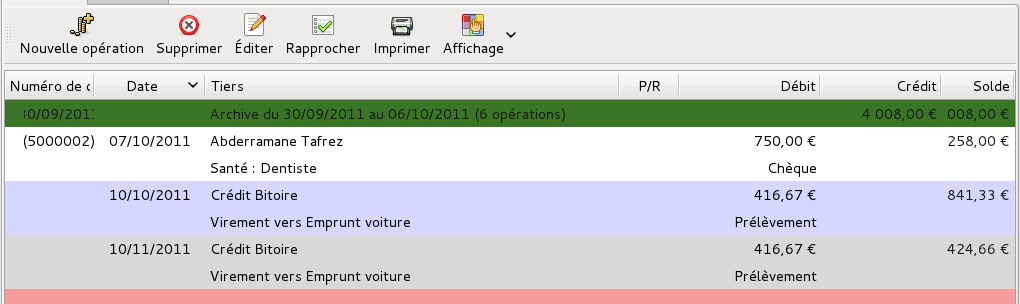
\includegraphics[scale=0.5]{image/screenshot/datamanagement_history_line}
\end{center}
\caption{Archive line displayed}
\label{datamanagement-history-line-img}
\end{figure}
% image centrée
\else the \indexword{ number of archived operations}\index{archive !nombre d'opérations} \emph{for the account displayed}, and the \indexword{total number of transactions}\index{opération !nombre total} in your accounts file.
\fi


You can show or hide all archive rows in the list of operations for all accounts by selecting the \menu{View - Show Lines Archive}, or by clicking the \menu{View} tool on the toolbar, and then click selecting \menu{Show Archive Lines} from its drop-down list.

If you want to view the operations inside an archive, you can open this archive by double-clicking on its line: after validation in the window that appears, the operations are displayed in the list.

\textbf{Note}: this is only an opening of the archive for display, and in no case this archive is deleted. The next time Grisbi is used, the green line of the archive will reappear at the top of the list for each account. For a true deletion of the archive, see the \vref{datamanagement-history-remove}, \menu{Deleting an archive} section.



\subsection{Creating and archive\label{datamanagement-history-new}}

To create an archive, follow these steps:

\begin{enumerate}
	\item in the menu bar, select \menu{File - Archive transactions\ldots{}} : The Archive Creation Wizard window is displayed; confirm with the \menu{Forward} button;
	\item in the following window, you can choose the operation selection mode to archive  \ifIllustration archiver\refimage{datamanagement-history-create-img}:
	% image centrée
	\begin{figure}[htbp]
	\begin{center}
	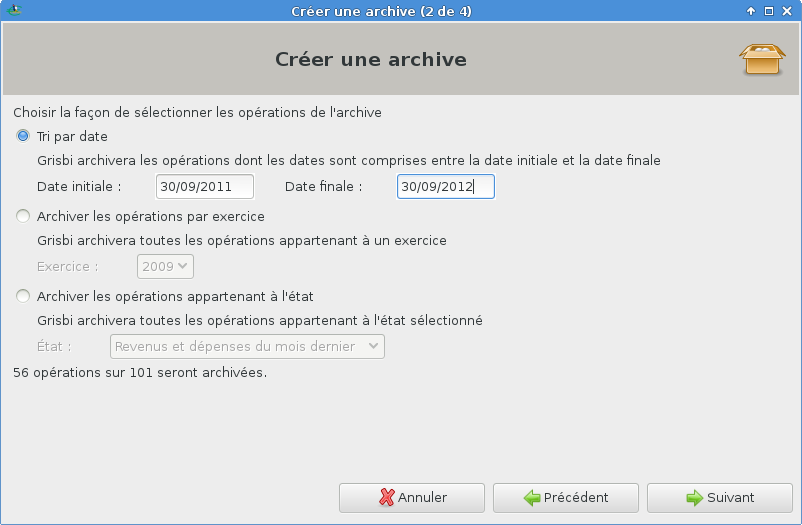
\includegraphics[scale=0.5]{image/screenshot/datamanagement_history_create}
	\end{center}
	\caption{Creating an archive}
	\label{datamanagement-history-create-img}
	\end{figure}
	% image centrée
	\else archiver :
	\fi
	
		\begin{itemize}
			\item \menu{Archive by Date}: enter the \menu{Initial date} and \menu{Final date} in the appropriate fields,
			\item \menu{Archive transactions by financial year}: Select an available year from the drop-down list,
			\item \menu{Archive transactions by report}: Select an available report from the drop-down list;
% saut de ligne pour indentation correcte de la note dans la liste

			\textbf{Note}: the last line in the window indicates either an error in entering these parameters, the number of transactions that will be archived and the total number of operations in your accounts file.  
		\end{itemize}
	\item confirm with the \menu{Forward} btton;
	\item in the next window, enter the name you want for this archive; confirm with the  \menu{Apply} button;
	\item the last window informs you that the archive has been created, and displays the \indexword{number of archived transactions}\index{archive !nombre d'opérations}, number of transactions and the total number of transactions of your accounts file;  \emph{all accounts taken together};  validate with the \menu{Back} button to create another archive, otherwise by the \menu{Close} button.
\end{enumerate}

\textbf{Note}: In case Grisbi has become slower after creating an archive, you can configure it to not load the close operations (R) on startup, in order to increase its speed, see the \ref{transactions-functions}, \menu{tool bar}).

% espace après Attention ou Note  : 5 mm
\vspacepdf{5mm}
The archive appears at the very top of the list of operations \emph{for each account} (see the \vref{datamanagement-history-list} section, \menu{Archives in the list of transactions}).


\subsection{Creation warning and automatic creation of archives\label{datamanagement-history-auto}}

When a certain number of registered transactions is reached, Grisbi can first of all warn you that this quantity of operations has not yet been archived, on the other hand automatically start the creation of an archive (see \vref{setup-general-archives-create}, \menu{warning and automatic creation}).

By clicking on the box labelled \menu{Automatically create an archive if necessary}, you enable the automatic archiving function.

With the label \menu{Warn if more transactions \ldots{ } are not archived}, you can set this number of operations. The default value is 3000.


\subsection{Parameters of an archive\label{datamanagement-history-parameters}}
You can consult the parameters that were defined during the creation of an archive, in the 
\menu{Edit - Preferences - Archives} menu. For this see the \vref{setup-general-archives-existing}, \menu{Existing Archives}.


\subsection{Editing an archive\label{datamanagement-history-modify}}

You can only \indexword{change the name of an archive}\index{archive !modification} in the \menu{Edit - Preferences } menu. For this see the \vref{setup-general-archives-remove}, \menu{Edit the archive} section.


\subsection{Deleting an archive\label{datamanagement-history-remove}}

You can \indexword{delete an existing archive}\index{archive !suppression} , in the menu \menu{Edit - Preferences} menu. There are two separate delete functions: deleting an archive while  \emph{retaining} its transactions,and deleting an archive while  \emph{deleting}  all its operations. For this see \vref{setup-general-archives-remove}, \menu{Edit the archive}. 


\subsection{Export an archive\label{datamanagement-history-export}}

Allows you to create a file containing the archive, in order to store it, or to use it in another Grisbi account file or in another accounting application. Exporting can only be done through \indexword{\gls{GSB}}\index{gsb}, \indexword{\gls{QIF}}\index{qif} or \indexword{\gls{CSV}}\index{csv}.

% espace avant Attention ou Note  : 5 mm
\vspacepdf{5mm}
\strong{Caution}: QIF and CSV file formats do not support currency, and all transactions will be converted to the currency of their respective account.
% espace après Attention ou Note  : 5 mm
\vspacepdf{5mm}



To export an archive, follow these steps:

\begin{enumerate}
	\item in the menu bar, select \menu{Export an archive to a GSB, QIF or CSV file ... } : the archive export wizard window is displayed; confirm with the \menu{Forward} button;
	\item a table displays the list of existing archives with their name and, as the case may be, their initial and final dates, their exercise or the name of the report; select the archive to export by checking the box in its line; confirm with the \menu{Forward} button;
	\item a file manager window is displayed; optionally modify the name of the file under which the archive will be exported, the folder where it will be saved and the format of the export file; confirm with the \menu{Forward} button;
	\item the last window informs you that the archive has been exported; confirm with the \menu{Close} button.
\end{enumerate}









